\section{Introduction}
\label{sec:Intro}

With the rapid development of deep learning, 
the medical influence community has also begun 
to try to apply this technology to improve the 
accuracy of cancer screening.
In the United States, breast cancer has become 
the second highest death rate among all cancers.
And screening mammography has become an 
effective way to reduce mortality.
According to a study by the Breast Cancer 
Surveillance Consortium in 2009, the overall 
sensitivity of digital screening mammography 
in the U.S. is 84.4$\%$ and the overall 
specificity is 90.8$\%$
\cite{Oeffinger2015}.  
Since the 1990s, the Computer-Assisted Detection 
and Diagnosis (CAD) software has been applied 
in clinical diagnosis, which can effectively 
help radiologists improve the efficiency of 
cancer detection. 
However, according to the actual situation 
of the application, this system is not as 
envisaged, the effect is not obvious, and 
there is no substantial progress in the 
upgrade and improvement of the system.
In recent years, deep learning has achieved 
better results in visual object recognition 
and detection, attracting more attention
\cite{Lecun2015}.
There is much more interest in deep learning 
to assist radiologists and improve the accuracy 
of screening mammography
\cite{Jamieson2012,Zhu2019,Shen2017}. 

Early detection of subclinical breast cancer 
on screening mammography is challenging as an 
image detection task because the tumors 
themselves occupy only a small portion of the 
image of the entire breast. 
For example, a full-field digital mammography 
(FFDM) image is typically 4000 × 3000 pixels 
while a cancerous region of interest (ROI) 
can be as small as 50 × 50 pixels. 
If ROI annotations were widely available in 
mammography databases then established object 
detection and classification methods such as 
the region-based convolutional neural network 
(R-CNN) and its variants could be readily 
applied
\cite{Girshick2014,Girshick2015,Ren2017}.
However, approaches that require ROI 
annotations often cannot be transferred to large mammography 
databases that lack ROI annotations, which are
laborious and costly to assemble
\cite{Dai2016}. 
Thus, it is essential to leverage both the few 
fully annotated datasets, as well as larger 
datasets labeled with only the cancer status 
of each image to improve the accuracy 
of breast cancer classification algorithms.

Pre-training is an effective way to train the 
network.
For example, use hierarchical pre-training to 
initialize the weight parameters of the DBN 
with hidden layers and then fine-tune them.
It is easy to find that pre-training can improve 
training speed and recognition accuracy. 
Another common method of training, first in 
large databases (such as ImageNet, and then 
fine-tune the model to complete other tasks
\cite{Russakovsky2015,9112355}.
Although certain tasks may be independent of 
the initial training data set, but the weight 
of the model parameters have been initialized 
weight, original features may be identified, 
which are easily used for other tasks.
This can often save training time and improve 
the performance of the model
\cite{He2016,Moreira2018}.


Inspired by \cite{Lin2020}, so and so.
to use the feature extraction capabilities 
of neural networks, researchers have recently 
proposed a new mammography recognition method.
However, we think that the underlying neural 
network capabilities to extratct image features 
can be better utilized.
In this study, different deep neural network 
models are merged to jointly propose a 
mammography image recognition method that can 
learn fine-grained mammography by fusing 
multiple functions.
In addition, the hash decoder method is used 
to simplify the classification calculation of 
complex high-dimensional feature vectors, 
and the results of different classifiers are 
merged at the end.
In summary, our work can be shown as follows:

1. Build a deep convolutional neural network based 
on well-performed network structures, and design a 
transfer learning strategy to improve the 
representation power of the extracted features.

2. To further utilize the feature representation 
ability of CNNs, we propose a method to fuse 
extracted features from multiple trained models 
with similar topological structure to
further improve the classification accuracy.

3. The strategy applied by hash learning in the 
deep network is cited to enhance the 
generalization ability of the model and solve the 
challenge of high-dimensional calculation 
in deep learning.

4. The designed feature fusion model is used in 
the feature extraction process of Faster RCNN, 
and a deep hash learning strategy is introduced 
in the classification stage.

This article is organized as follows. 
Section~\ref{sec:Meth} 
details of the network structure and the proposed 
method. 
Section~\ref{sec:Data} 
elaborates the dataset used in our work.
Section~\ref{sec:Exp} 
shows experimental results demonstrate, and 
given the discussion.
Section~\ref{sec:Conc} 
makes the conclusion and future work are provided 
in the end.

\begin{figure*}[!ht]
    \centering
    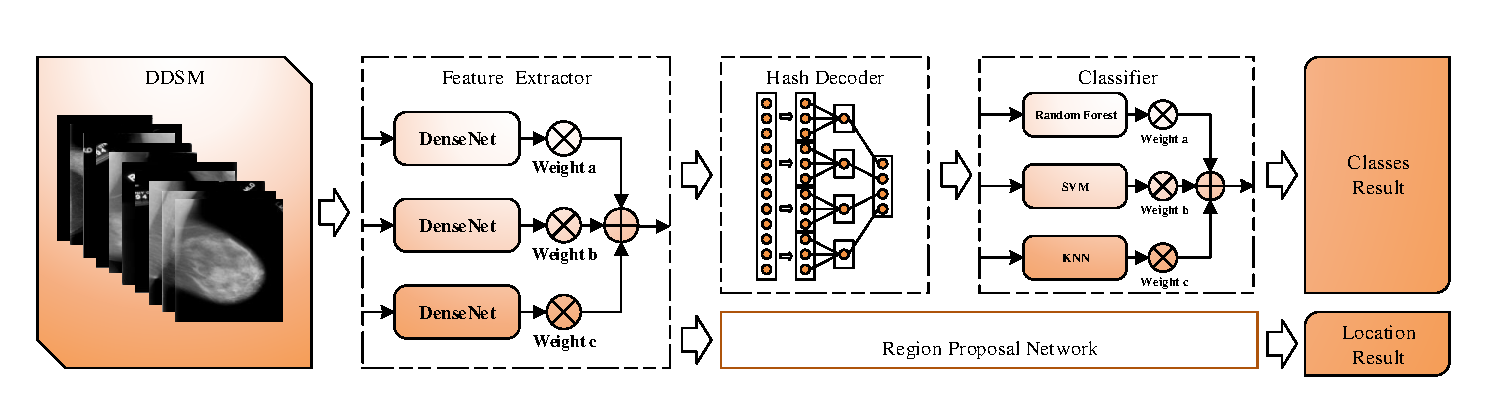
\includegraphics[
        width=1.0\textwidth,
        keepaspectratio
    ]{NetStruct.pdf}
    \caption{Overview of the proposed approach.}
    \label{fig:netStruct}
\end{figure*}
